\documentclass{article}

\usepackage{amsmath}
\usepackage[english]{babel}
\usepackage{blindtext}
\usepackage{setspace}
\usepackage{graphicx}
\usepackage[utf8]{inputenc}
\usepackage{fancyhdr}
\usepackage{array}
\usepackage[table]{xcolor}
\usepackage{subfiles}
\usepackage{multicol}
\usepackage[bottom]{footmisc}
\usepackage{amsfonts}
\usepackage{pgfplots} 
\usepackage{longdivision}
\usepackage{polynom}
\usepackage{hyperref}
\pgfplotsset{width=9cm,compat=1.9}

\begin{document}
\pagenumbering{gobble}

\begin{center}
    \vspace*{-2cm}
    
\includegraphics[width=3cm]{../../Images/Stiftelsen_Logo.jpg}
\end{center}
\vspace{1.5cm}

\fontfamily{phv}

\noindent
\textbf{\begin{Huge}Sorteringsalgoritmer\end{Huge}}\\
\vspace{0.2cm}
\begin{LARGE}Analys av sorteringsalgoritmer med C\#\end{LARGE}\\
\rule[0.3cm]{\linewidth}{1pt}
\Large
\noindent
\textit{Analysis of comparative sorting algorithms within C\#}
\vspace{1cm}
\vspace{1cm}
\noindent
\LARGE
Erik V Norberg, Sci18\\
\vspace{4 cm}
\small
\par \noindent
Gymnasiearbete
\par \noindent
Europaskolan Strängnäs
\par \noindent
Naturvetenskapliga programmet
\par \noindent
Handledare: Johan Wild
\par \noindent
Ht20 - Vt21

% Adds background picture. Delete code if no background picture is wanted.
\begin{tikzpicture}[overlay, remember picture]
    \node[anchor=south west, 
          xshift=-0.2cm, 
          yshift=-0.2cm] 
         at (current page.south west)
         {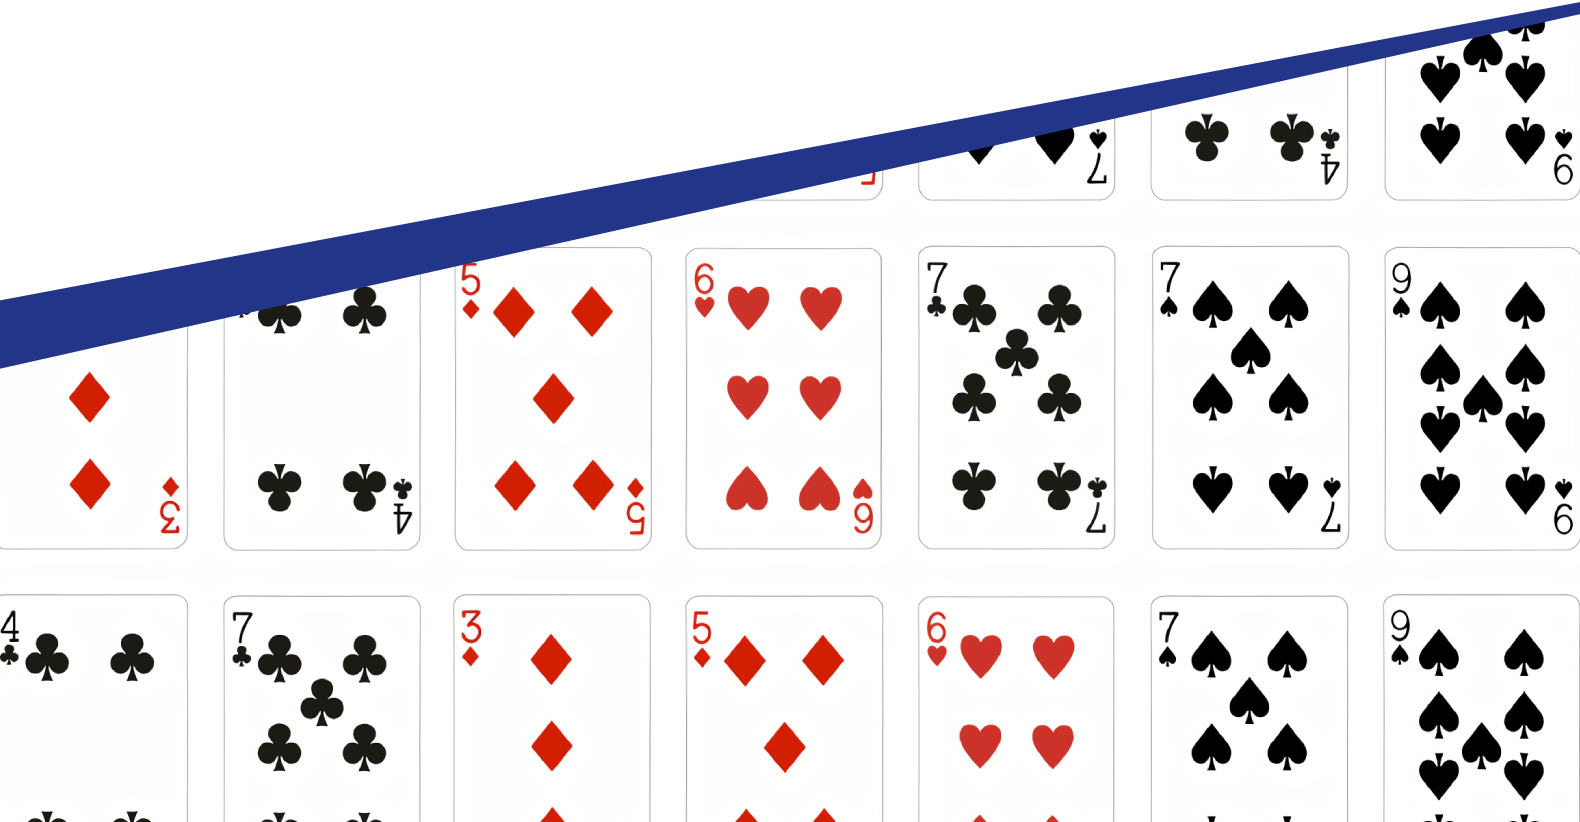
\includegraphics[width = 1.8\textwidth, height = 10cm]{../../Images/Background.png}}; 
\end{tikzpicture}

\newpage
\textcolor{white}{temp}

\end{document}